% Also note that the "draftcls" or "draftclsnofoot", not "draft", option
% should be used if it is desired that the figures are to be displayed in
% draft mode.

\documentclass[conference]{IEEEtran}
% Add the compsoc option for Computer Society conferences.
%
% If IEEEtran.cls has not been installed into the LaTeX system files,
% manually specify the path to it like:
% \documentclass[conference]{../sty/IEEEtran}

	% Some very useful LaTeX packages include:
	% (uncomment the ones you want to load)

	% *** MISC UTILITY PACKAGES ***
	%\usepackage{ifpdf}
		% Heiko Oberdiek's ifpdf.sty is very useful if you need conditional compilation based on whether 
		% the output is pdf or dvi.
		% usage:
		% \ifpdf
		%   % pdf code
		% \else
		%   % dvi code
		% \fi
		% The latest version of ifpdf.sty can be obtained from: http://www.ctan.org/tex-archive/macros/latex/contrib/oberdiek/
		% Also, note that IEEEtran.cls V1.7 and later provides a builtin \ifCLASSINFOpdf conditional that 
		% works the same way. When switching from latex to pdflatex and vice-versa, the compiler may
		% have to be run twice to clear warning/error messages.

	% *** CITATION PACKAGES ***
	\usepackage{cite}
		% cite.sty was written by Donald Arseneau
		% V1.6 and later of IEEEtran pre-defines the format of the cite.sty package
		% \cite{} output to follow that of IEEE. Loading the cite package will
		% result in citation numbers being automatically sorted and properly
		% "compressed/ranged". e.g., [1], [9], [2], [7], [5], [6] without using
		% cite.sty will become [1], [2], [5]--[7], [9] using cite.sty. cite.sty's
		% \cite will automatically add leading space, if needed. Use cite.sty's
		% noadjust option (cite.sty V3.8 and later) if you want to turn this off.
		% cite.sty is already installed on most LaTeX systems. Be sure and use
		% version 4.0 (2003-05-27) and later if using hyperref.sty. cite.sty does
		% not currently provide for hyperlinked citations.
		% The latest version can be obtained at:
		% http://www.ctan.org/tex-archive/macros/latex/contrib/cite/
		% The documentation is contained in the cite.sty file itself.

	% *** GRAPHICS RELATED PACKAGES ***
	\ifCLASSINFOpdf
		\usepackage[pdftex]{graphicx}
			% declare the path(s) where your graphic files are
			% \graphicspath{{../pdf/}{../jpeg/}}
			% and their extensions so you won't have to specify these with
			% every instance of \includegraphics
			% \DeclareGraphicsExtensions{.pdf,.jpeg,.png}
	\else
		% or other class option (dvipsone, dvipdf, if not using dvips). graphicx
		% will default to the driver specified in the system graphics.cfg if no
		% driver is specified.
		% \usepackage[dvips]{graphicx}
		% declare the path(s) where your graphic files are
		% \graphicspath{{../eps/}}
		% and their extensions so you won't have to specify these with
		% every instance of \includegraphics
		% \DeclareGraphicsExtensions{.eps}
	\fi
		% graphicx was written by David Carlisle and Sebastian Rahtz. It is
		% required if you want graphics, photos, etc. graphicx.sty is already
		% installed on most LaTeX systems. The latest version and documentation can
		% be obtained at: 
		% http://www.ctan.org/tex-archive/macros/latex/required/graphics/
		% Another good source of documentation is "Using Imported Graphics in
		% LaTeX2e" by Keith Reckdahl which can be found as epslatex.ps or
		% epslatex.pdf at: http://www.ctan.org/tex-archive/info/
		% latex, and pdflatex in dvi mode, support graphics in encapsulated
		% postscript (.eps) format. pdflatex in pdf mode supports graphics
		% in .pdf, .jpeg, .png and .mps (metapost) formats. Users should ensure
		% that all non-photo figures use a vector format (.eps, .pdf, .mps) and
		% not a bitmapped formats (.jpeg, .png). IEEE frowns on bitmapped formats
		% which can result in "jaggedy"/blurry rendering of lines and letters as
		% well as large increases in file sizes.
		% You can find documentation about the pdfTeX application at:
		% http://www.tug.org/applications/pdftex

	% *** MATH PACKAGES ***
	\usepackage[cmex10]{amsmath}
		% A popular package from the American Mathematical Society that provides
		% many useful and powerful commands for dealing with mathematics. If using
		% it, be sure to load this package with the cmex10 option to ensure that
		% only type 1 fonts will utilized at all point sizes. Without this option,
		% it is possible that some math symbols, particularly those within
		% footnotes, will be rendered in bitmap form which will result in a
		% document that can not be IEEE Xplore compliant!
		%
		% Also, note that the amsmath package sets \interdisplaylinepenalty to 10000
		% thus preventing page breaks from occurring within multiline equations. Use:
		%\interdisplaylinepenalty=2500
		% after loading amsmath to restore such page breaks as IEEEtran.cls normally
		% does. amsmath.sty is already installed on most LaTeX systems. The latest
		% version and documentation can be obtained at:
		% http://www.ctan.org/tex-archive/macros/latex/required/amslatex/math/
	\usepackage{amssymb}

	% *** SPECIALIZED LIST PACKAGES ***
	\usepackage{algorithmic}
		% algorithmic.sty was written by Peter Williams and Rogerio Brito.
		% This package provides an algorithmic environment fo describing algorithms.
		% You can use the algorithmic environment in-text or within a figure
		% environment to provide for a floating algorithm. Do NOT use the algorithm
		% floating environment provided by algorithm.sty (by the same authors) or
		% algorithm2e.sty (by Christophe Fiorio) as IEEE does not use dedicated
		% algorithm float types and packages that provide these will not provide
		% correct IEEE style captions. The latest version and documentation of
		% algorithmic.sty can be obtained at:
		% http://www.ctan.org/tex-archive/macros/latex/contrib/algorithms/
		% There is also a support site at:
		% http://algorithms.berlios.de/index.html
		% Also of interest may be the (relatively newer and more customizable)
		% algorithmicx.sty package by Szasz Janos:
		% http://www.ctan.org/tex-archive/macros/latex/contrib/algorithmicx/

	% *** ALIGNMENT PACKAGES ***
	\usepackage{array}
		% Frank Mittelbach's and David Carlisle's array.sty patches and improves
		% the standard LaTeX2e array and tabular environments to provide better
		% appearance and additional user controls. As the default LaTeX2e table
		% generation code is lacking to the point of almost being broken with
		% respect to the quality of the end results, all users are strongly
		% advised to use an enhanced (at the very least that provided by array.sty)
		% set of table tools. array.sty is already installed on most systems. The
		% latest version and documentation can be obtained at:
		% http://www.ctan.org/tex-archive/macros/latex/required/tools/
	\usepackage{mdwmath}
	\usepackage{mdwtab}
		% Also highly recommended is Mark Wooding's extremely powerful MDW tools,
		% especially mdwmath.sty and mdwtab.sty which are used to format equations
		% and tables, respectively. The MDWtools set is already installed on most
		% LaTeX systems. The lastest version and documentation is available at:
		% http://www.ctan.org/tex-archive/macros/latex/contrib/mdwtools/
		% IEEEtran contains the IEEEeqnarray family of commands that can be used to
		% generate multiline equations as well as matrices, tables, etc., of high
		% quality.
	\usepackage{eqparbox}
		% Also of notable interest is Scott Pakin's eqparbox package for creating
		% (automatically sized) equal width boxes - aka "natural width parboxes".
		% Available at:
		% http://www.ctan.org/tex-archive/macros/latex/contrib/eqparbox/

	% *** SUBFIGURE PACKAGES ***
	%\usepackage[tight,footnotesize]{subfigure}
		% subfigure.sty was written by Steven Douglas Cochran. This package makes it
		% easy to put subfigures in your figures. e.g., "Figure 1a and 1b". For IEEE
		% work, it is a good idea to load it with the tight package option to reduce
		% the amount of white space around the subfigures. subfigure.sty is already
		% installed on most LaTeX systems. The latest version and documentation can
		% be obtained at:
		% http://www.ctan.org/tex-archive/obsolete/macros/latex/contrib/subfigure/
		% subfigure.sty has been superceeded by subfig.sty.
	%\usepackage[caption=false]{caption}
	%\usepackage[font=footnotesize]{subfig}
		% subfig.sty, also written by Steven Douglas Cochran, is the modern
		% replacement for subfigure.sty. However, subfig.sty requires and
		% automatically loads Axel Sommerfeldt's caption.sty which will override
		% IEEEtran.cls handling of captions and this will result in nonIEEE style
		% figure/table captions. To prevent this problem, be sure and preload
		% caption.sty with its "caption=false" package option. This is will preserve
		% IEEEtran.cls handing of captions. Version 1.3 (2005/06/28) and later 
		% (recommended due to many improvements over 1.2) of subfig.sty supports
		% the caption=false option directly:
	%\usepackage[caption=false,font=footnotesize]{subfig}
		% The latest version and documentation can be obtained at:
		% http://www.ctan.org/tex-archive/macros/latex/contrib/subfig/
		% The latest version and documentation of caption.sty can be obtained at:
		% http://www.ctan.org/tex-archive/macros/latex/contrib/caption/

	% *** FLOAT PACKAGES ***
	%\usepackage{fixltx2e}
		% fixltx2e, the successor to the earlier fix2col.sty, was written by
		% Frank Mittelbach and David Carlisle. This package corrects a few problems
		% in the LaTeX2e kernel, the most notable of which is that in current
		% LaTeX2e releases, the ordering of single and double column floats is not
		% guaranteed to be preserved. Thus, an unpatched LaTeX2e can allow a
		% single column figure to be placed prior to an earlier double column
		% figure. The latest version and documentation can be found at:
		% http://www.ctan.org/tex-archive/macros/latex/base/
	%\usepackage{stfloats}
		% stfloats.sty was written by Sigitas Tolusis. This package gives LaTeX2e
		% the ability to do double column floats at the bottom of the page as well
		% as the top. (e.g., "\begin{figure*}[!b]" is not normally possible in
		% LaTeX2e). It also provides a command:
		%\fnbelowfloat
		% to enable the placement of footnotes below bottom floats (the standard
		% LaTeX2e kernel puts them above bottom floats). This is an invasive package
		% which rewrites many portions of the LaTeX2e float routines. It may not work
		% with other packages that modify the LaTeX2e float routines. The latest
		% version and documentation can be obtained at:
		% http://www.ctan.org/tex-archive/macros/latex/contrib/sttools/
		% Documentation is contained in the stfloats.sty comments as well as in the
		% presfull.pdf file. Do not use the stfloats baselinefloat ability as IEEE
		% does not allow \baselineskip to stretch. Authors submitting work to the
		% IEEE should note that IEEE rarely uses double column equations and
		% that authors should try to avoid such use. Do not be tempted to use the
		% cuted.sty or midfloat.sty packages (also by Sigitas Tolusis) as IEEE does
		% not format its papers in such ways.

	% *** PDF, URL AND HYPERLINK PACKAGES ***
	%\usepackage{url}
		% url.sty was written by Donald Arseneau. It provides better support for
		% handling and breaking URLs. url.sty is already installed on most LaTeX
		% systems. The latest version can be obtained at:
		% http://www.ctan.org/tex-archive/macros/latex/contrib/misc/
		% Read the url.sty source comments for usage information. Basically,
		% \url{my_url_here}.
		% *** Do not adjust lengths that control margins, column widths, etc. ***
		% *** Do not use packages that alter fonts (such as pslatex).         ***
		% There should be no need to do such things with IEEEtran.cls V1.6 and later.
		% (Unless specifically asked to do so by the journal or conference you plan
		% to submit to, of course. )

	% *** LANGUAGE PACKAGES ***
		\usepackage[latin1]{inputenc}
		\usepackage[english]{babel}

%	CORRECTION FOR HYPERNATION	
	\hyphenation{op-tical net-works semi-conduc-tor tran-si-cio-nes}

%	DOCUMENT BEGINING
	\begin{document}		
	
	%	TITLE AND AUTHORS
		%	TITLE
	% paper title
	% can use linebreaks \\ within to get better formatting as desired
		\title{Execution of Timed Petri Nets with IP cores}

%	AUTHORS
	% author names and affiliations
	% use a multiple column layout for up to three different affiliations

	% conference papers do not typically use \thanks and this command
	% is locked out in conference mode. If really needed, such as for
	% the acknowledgment of grants, issue a \IEEEoverridecommandlockouts
	% after \documentclass

	% for over three affiliations, or if they all won't fit within the width
	% of the page, use this alternative format:
	% 
	\author{
		\IEEEauthorblockN{Orlando Micolini}
		\IEEEauthorblockA{
			Laboratorio de Arquitectura \\ de Computadoras\\
			FCEFyN-UNC\\
			C�rdoba, Argentina\\
			Email: omicolini@compuar.com
		}	
	\and
		\IEEEauthorblockN{Julian Nonino}
		\IEEEauthorblockA{
			Laboratorio de Arquitectura \\ de Computadoras\\
			FCEFyN-UNC\\
			C�rdoba, Argentina\\
			Email: noninojulian@gmail.com
		}	
		\and
		\IEEEauthorblockN{Carlos Renzo Pisetta}
		\IEEEauthorblockA{
			Laboratorio de Arquitectura \\ de Computadoras\\
			FCEFyN-UNC\\
			C�rdoba, Argentina\\
			Email: renzopisetta@gmail.com
		}	
	}

	% use for special paper notices
	%\IEEEspecialpapernotice{(Invited Paper)}

	% make the title area
		\maketitle
		
	% For peer review papers, you can put extra information on the cover
	% page as needed:
	% \ifCLASSOPTIONpeerreview
	% \begin{center} \bfseries EDICS Category: 3-BBND \end{center}
	% \fi
	%
	% For peerreview papers, this IEEEtran command inserts a page break and
	% creates the second title. It will be ignored for other modes.
		\IEEEpeerreviewmaketitle
		
	%	ABSTRACT
		\begin{abstract}
	%\boldmath.
	
	In this article, we present a Timed Petri Nets processor wich can be can be directly programmed 
	using vectors and matrices of Petri Nets formalism. This processor can leverage the power of Petri
	Nets for modeling real-time systems and formally verify their properties, which prevent programming
	errors.
	\\
	
	The Petri Nets processor was developed as an IP-core to be inserted in a multi-core system.
	Therefore, we can model the system requirements with Petri Nets, formally verifying all its
	properties and using the IP-core to implement the system is possible to ensure that all properties
	will be met.
	
\end{abstract}
% IEEEtran.cls defaults to using nonbold math in the Abstract.
% This preserves the distinction between vectors and scalars. However,
% if the conference you are submitting to favors bold math in the abstract,
% then you can use LaTeX's standard command \boldmath at the very start
% of the abstract to achieve this. Many IEEE journals/conferences frown on
% math in the abstract anyway.

\begin{IEEEkeywords}
	Multi-Core, Petri Net, Processor.
\end{IEEEkeywords}

	%	INTRODUCTION
		\section{Introduction}
	\IEEEPARstart{T}{he} computer systems are complex as much its structure as its behavior, even 
	more when they have a great number of states and many combinations of data and input events.

Develop solutions of complex and critical systems for give a solution a real-time systems have 
 problems such as: the inherent complexity of the specification, the coordination of concurrent 
 tasks, the lack of portable algorithms, standardized environments, software and development tools.

And taking into account unambiguous trends in the hardware design, which indicate that one processor
 may not be able to keep pace with increase performance. Therefore the evolution of the processors 
 is consequence of the greater integration and composition of different types of functionalities 
 integrated into a single processor. Even more today, the availability of transistors has made 
 possible to integrate several processor cores on a single chip, which has resulted in the 
 development of Multi-Core technology \cite{hennessypatterson}.
 
Diminishing returns of Instruction Level Parallelism (ILP) and the cost of the increase of frequency,
 mainly due to power limitations (suggests that a 1\% increase in clock speed results in a power 
 increase of 3\%) \cite{domeika}, leads to the use of multicore processors to improve performance. 
 This increase deficiency results in lower run times, lower consumption, lower energy density, lower
 latency and higher bandwidth inter-core communications.
    
Therefore multi-core processors are a proposal to obtain higher performance. This mainly involves 
 lower execution time, energy consumption, energy density, latency and more bandwidth inter-core 
 communications. Furthermore, the heterogeneous multi-core systems have the advantage of employing 
 specialized cores, each of them designed for specific tasks. That is, optimized for a particular 
 need. These processors have the ability to use the available hardware resources when they are 
 specifically required by the software \cite{sriram}.

In order to increase performance, these systems make use of multi-threading and/or multi-tasking 
 allowing take advantage of the multi-cores. However, it takes more effort to design applications 
 because they must provide solution to the problems of concurrent systems.

That is the reason why with these processors, the parallel programming is essential for improving 
 the performance in all segments of software development and even more so in the segment of real-time
 systems.
 
At the Computer Architectures Laboratory of the FCEFyN-UNC a Petri processor has been developed to 
 directly execute ordinary Petri Nets. In this article, we present a new Petri Nets Processor capable
 to execute Time Petri Nets and to be programmed directly with the vectors and matrixes that define 
 the system and its state.
	


	
	%	OBJECTIVES
		\section{Objectives}

	\subsection{Main Objective}
	
		The main objective of this work is to design and implement a Petri Nets Processor capable 
		to execute the Timed Petri Nets semantics and to be programmed directly from the model\'s 
		state equations.
	
	\subsection{Secondary Objectives}
	
		The secondary objectives are:
		\begin{itemize}
		  	\item Briefly describe Timed Petri Nets in order to implement a processor capable of execute 
		  		them.
		  	\item Keep executing ordinary Petri Nets with time parameters on two processor clock cycles.
		  	\item Implement the Timed Petri Nets processor as an IP-core.
		\end{itemize}
		

	%	PETRI NETS CONSIDERING TIME
		\section{Petri Nets Considering Time}
	
	In the Ordinary Petri Nets formalism, the time is not consider and this results in indeterminism 
	regarding the time. It is not specified when a sensibilized transition will be fired or even if it
	will be fired. Neither can be said which transition from a group of transitions in conflict will 
	be fired \cite{garciaizquierdo}.
	
	There are three different interpretations about how the time should be consider. All of them have 
	focus on reduce the indeterminism regarding time in Petri Nets.
	\begin{enumerate}
	  	\renewcommand{\theenumi}{\Alph{enumi}}
	  	\item \underline{Stochastic Petri Net}
	  		\\
			Introduces a stochastic estimation on the instant of firing of a transition.
		\item \underline{Timed Petri Net}
			\\
			Introduces a time condition which specifies the duration of the transition.
		\item \underline{Time Petri Net}
			\\
			Introduce temporary dimensions between which the transition should be fired.
	\end{enumerate}
		
	\begin{figure}[h]
		\centering
		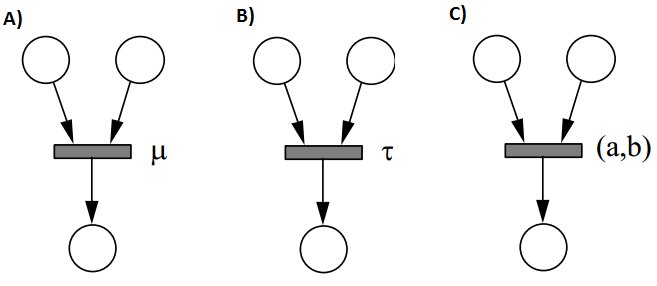
\includegraphics[width=1\linewidth]{./img/Petri16}
		\caption{Different ways to intruduce time in Petri Nets}
		\label{fig:Petri16}
	\end{figure}
	
	The temporal parameters associated with transitions can be interpreted in these three different
	ways\footnotemark:
	
	\footnotetext{ $\bullet t$ is the set of places that are inputs to a
	transition, mathematically defined as: $\bullet t = \{ p \in P : (p , t) \in F \}$.
	
	$t \bullet$ is the set of positions that are outputs of a transition, mathematically defined as: 
		$t \bullet = \{ p \in P : (t , p) \in F \}$.
	
	$F$ is the set of arcs, input and output to the transitions-
	}	
	
	\begin{enumerate}
	  	\item Generalised Stochastic Petri Nets (GSPNs) \cite{gspn} have two different types of 
	  		transitions: immediate transitions and timed transitions. When a transition \emph{t} is
	  		sensitized, its firing could be:
			\begin{enumerate}
			  	\item with a duration equal to zero if the transition \emph{t} is immediate.
			  	\item after lapse of a random time. This random time is expressed by an exponential 
			  	distribution. The A net from the figure \ref{fig:Petri16} graphically represents an stochastic
			  	timed transition where its probability to be fired is represented by $\mu$.
			\end{enumerate}
		\item Timed Petri Nets have two different types of transitions: immediate transitions and timed
			transitions. When a transition \emph{t} is sensitized, its firing could be:
			\begin{enumerate}
			  	\item with a duration equal to zero if the transition \emph{t} is immediate.
			  	\item with immediate removal of tokens from $\bullet t$ set but placing the tokens in 
			  	the $t \bullet$ that only after time $\tau$ has elapsed. Meanwhile, the transition 
			  	can not be sensitized. The B net from the figure \ref{fig:Petri16} graphically represents 
			  	a timed transition with a delay equal to $\tau$.
			\end{enumerate}
		\item Timed Petri Nets have two different types of transitions: immediate transitions and time
			transitions. When a transition \emph{t} is sensitized, its firing could be:
			\begin{enumerate}
			  	\item with a duration equal to zero if the transition \emph{t} is immediate.
			  	\item if it is a time transition, at the time it is sensitized, a timer stars. The transition
			  	can only be fired when the timer value is between the limits of the interval [a, b].
			  	Otherwise, the transition can not be fired. Once the firing was performed, the timer is
			  	restarted. The C net from the figure \ref{fig:Petri16} graphically represents  a time transition
			  	with an associated interval equal to [a, b].
			\end{enumerate}		
	\end{enumerate}
	
	Should be noted that all the firings are performed in two steps.
	\begin{enumerate}
		\item The removal of the tokens from the $\bullet t$ set. This is an atomica action and the amount
			of tokens removed from each place is equal to the weight of the arcs joining each place $p \in
			\bullet t$ with the transition $t$.
		\item The atomic action of placing in each place of $t \bullet$ set the amount of tokens indicated
			by the weight of the arcs joining each place $p \in t \bullet$ with the transition $t$..
	\end{enumerate}
	
		
	%	TIME PETRI NETS
		\section{Timed Petri Nets}
\label{sec:timed_petri_nets}
	In this nets, each timed transition has an associated a parameter $\tau$ which represents
	the duration of the transition. In order to standardize the mathematical definition we will call 
	\emph{immediate} to those transitions where $\tau$ is zero.
	
	\subsection{Mathematical Definition}
		A \emph{Marked Timed Petri Net} \cite{garciaizquierdo}, is mathematically defined as a 8-tuple as follows:
		\begin{equation*}
			PN = \{P, T, I^-, I^+, H, C, m_0, \Gamma\}
		\end{equation*}
		Where the terms $\{P, T, I^-, I^+, H, C, m_0\}$ represent a marked Petri Net with inhibitors 
		arms and bounded places. $\Gamma$ is a vector composed of the values of duration $\tau$
		associated to each transition.
		
		The meaning of each term of the tuple is:		  
		\begin{itemize}
			\item \textbf{P} is a non-empty finite set of places.
			\item \textbf{T} is a non-empty finite set of transitions.
			\item \textbf{$I^+$} and \textbf{$I^-$} are the possitive and negative incidence matrices.
				\begin{equation*}
					P�T\rightarrow \mathbb{Z}
				\end{equation*}
			\item \textbf{H} is the inhibitors arcs matrix.
				$P�T\rightarrow\{0,1\}$
			\item $m_0$ is the net initial marking.
				$P\rightarrow \mathbb{N}$
			\item $C$ is a vector containing the values that represent the maximum amount of tokens
				that each place of the net can hold.
				$C\rightarrow \mathbb{N}$	
			\item \textbf{$\Gamma$} is the set of static intervals associated with each transition. 
				$T\rightarrow \mathbb{Q}^+ � (\mathbb{Q}^+ \cup \infty)$	
				For each transition \emph{t} the associated value $timer_t$ is:
				\begin{equation*}
					\Gamma (t) = (tau_t \text{ where } t \in T \text{ and } \tau \rightarrow \mathbb{Q}^+
				\end{equation*}
		\end{itemize}
		
		$timer_t$ represents the time elapsed since the firing of the transition start and its value 
		its value is zero at any other moment. $\tau_t$ is the duration of the transition. For that
		reasons, the following conditions must be met:
		\begin{equation*}
			\begin{matrix}
				0 \leq timer_t \leq \tau_t
				\\
				0 \leq \tau_t \leq \infty
			\end{matrix}
		\end{equation*}
		
	\subsection{States of a Timed Petri Net}
		
		In these Petri Nets, the net state is defined by the marking vector ($m=i$) and an 
		\emph{timer} vector that indicates the time stamp of each trasition. Therefore the net 
		state is:
		\begin{equation*}
			S = (m_i,\tau)
			\label{eq:timed_net_state}
		\end{equation*}
			
	\subsection{Sensitization of the Transitions and Firing Rules}
	\label{subsec:sensitization_transitions}
%TODO translate this		
		When we refer to transitions we need to establish the diference between an  enabled or sensitized 
		transition, a not enabled or sensitized transition  and the firing of a transition.

		In a Marked Petri Net whose current mark is $m_k$  we say that a transition $t_j$ is enabled or
		sensitized if and only if $timer_{tj}=0$ and the amount of tokens in all places $p_i$ belonging to
		the set $\bullet t_j$ is at least equal to the weight of the arc that connects them with the
		transition $t_j$ ($w(p_i , t_j)$). Mathematically:
		\begin{equation*}
			\forall p_i \in \bullet t_j : m(p_i) \geq w(p_i,t_j ) \land timer_{tj}=0
			\label{eq:sensitization_conditions}
		\end{equation*}
		
		In summary, every place connected to the transition $t_j$ have at least the number of tokens 
		indicated by the weight of the arc and there is no firing in progress for that transition.
		
		Sensitized transitions can be fired and every time the firing of a transition is completed it
		generates a new marking for the Petri Net. This means that the net changes its state.

		To determine the new state or mark of the net after firing a transition $t_j$, you should the
		\emph{state equation} $\delta(m_k , t_j)$.
		
		\begin{equation*}	
			\delta (m_k,t_j)
				\begin{cases} 
					m_{k+1} (p_i)=m_k (p_i )-W_{ij} & \forall p_i \in \bullet t_j 
					\\ 
					m_{k+1} (p_i)=m_k (p_i )+W_{ij} & \forall p_i \in t_j \bullet \land timer_{tj}=\tau_tj
					\\
					m_{k+1} (p_i)=m_k (p_i ) & \mbox{in the rest of the cases}
				\end{cases}
			\label{eq:state_equations}
		\end{equation*}

		$timer_{tj}$ is incremented in every clock cycle after the firing of the transition started.

	\subsection{Interpretation of the firing of transitions in the system}
		The figure \ref{fig:reactive_systems} represents a reactive systems that responds to events which
		come from the environment, it interacs with the environment. Those events are directed to the Time
		Petri Nets processor.
	
		The responsibility of the processor is arrange events  according to system constraints. These
		constraints are modeled by the TImed Petri Net which is used to program the processor. On the
		other hand, multicore system threads also generate events (to request resources, to synchronize) 
		that are directed to the processor.		
		\begin{figure}[h]
			\centering
			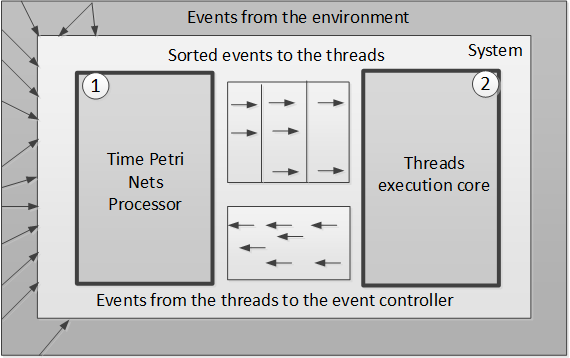
\includegraphics[width=1\linewidth]{./img/reactive_system}
			\caption{Reactive systems}
			\label{fig:reactive_systems}
		\end{figure}
		
		Module 1 from the Figure \ref{fig:reactive_systems} receive unsorted events from the environment
		and from the system itself. After the sorting of the events the Timed Petri Nets processor
		transmits the result to the threads execution cores (module 2) of the system and the propers
		actions are taken. 
			
%TODO No se entiende el significado
\textbf{
No se entiende el significado
\\
Si en nuestro  sistema se asocian el cumplimiento de las condiciones del programa a las que las transiciones 
est�n sensibilizadas, la resoluci�n de un disparo  representaran el cumplimiento de dichas restricciones y si 
asociamos la solicitud de verificaci�n de las condiciones a la solicitud de un disparo, la resoluci�n de un 
disparo comunica que las condiciones se han cumplido.
}		
		
		The conditions to be met for the firing of a transition from Timed Petri Processor are:
		\begin{enumerate}
			\item The transition must comply with sensitization conditions named in Section
				\ref{subsec:sensitization_transitions}.
			\item The shot must be explicitly communicated to the processes or implicitly recorded in the
				module of systolic firings.
			\item Since it is possible that multiple transitions simultaneously satisfy the conditions
				described in paragraphs 1 and 2, the Timed Petri Nets processor will execute first the
				firing with higher priority.
		\end{enumerate}	

		Figure \ref{fig:conection_multicore_system} show us how the Timed Petri Nets processor is conected
		in a multicore system.
	
		In case that the firing of the transition can not be resolve, it is queued in the input queue, as
		shown in Figure \ref{fig:conection_multicore_system}, until the conditions of the system allow
		its resolution. The solution of the firing is notified to threads through the system bus, using
		the output queue. The threads of the system will execute the proper actions as indicated by the
		firings that have been resolved, since the resoluction of the firings depends on the Time Petri
		Nets processor state, which itself represents the state of the system.
	
		\begin{figure}[h]
			\centering
			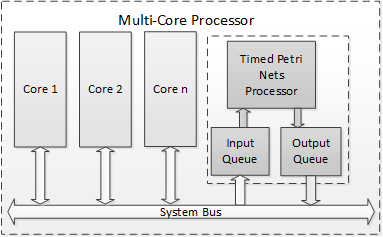
\includegraphics[width=1\linewidth]{./img/conection_multicore_system}
			\caption{Multicore system with Timed Petri Nets processor}
			\label{fig:conection_multicore_system}
		\end{figure}		
		
		
	%	TIMED PETRI PROCESSOR ARCHITECTURE AND OPERATION 
		\section{Timed Petri Nets Processor Architecture and Operation}

	The processor executes the state equation solving only a firing of a transition at a time, this
	way can solve all cases of firings, the simple ones (single firings) and the multiple firings,
	performing as a single-firing sequence, as a result, the hardware is simpler.
	
	The resolution of firings is requested by the threads running on the cores through the system bus,
	as emerging requests that system is running. These firing requests are received by the Timed Petri
	processor and stored in the input queue. This queue is FIFO according to each transition, the
	output of this queue is a binary word of size equal to the number of transitions. This word has
	\emph{ones} in the positions corresponding to transitions with firings requested. The order of the
	bit in the word equals the number of transition over which the firing is requested. The bits that
	correspond to the transitions which has no firing request are \emph{zero}.
	
	The output queue has a similar structure, but its function is to communicate to the threads those
	firings that have been resolved.
	
	\begin{figure}[h]
        \centering
        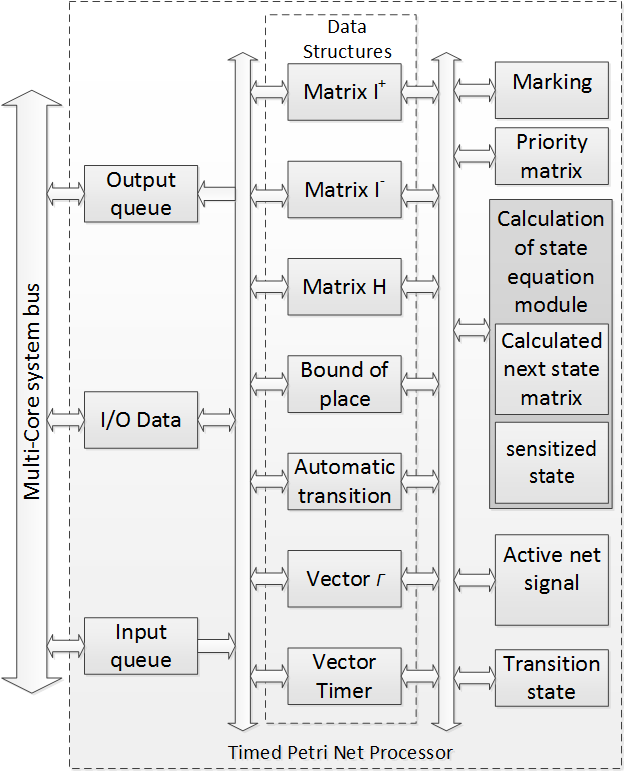
\includegraphics[width=1\linewidth]{./img/timed_petri_nets_processor}
        \caption{Timed Petri Nets Processor}
        \label{fig:time_petri_nets_processor}
    \end{figure}
	
    The data I/O module manages the access of the cores to the matrices and vectors that program the 
    system. The module manages the access of the cores to the matrices and vectors that program the 
    system.
    
    The matrices and vectors described in the equation of state are the system program. This allows 
    us to program the processor directly from the Timed Petri Net.

    Here we have added the inhibitor arcs matrix and the vector indicating the maximum number of tokens 
    in the places. This terms are not present in the state equitions shown in this work but you can 
    consult the work \cite{micolinipereyragalliaalasia} to obtain more information about those elements.

    The module in charge of solving the state equation of the Petri has the following responsabilities:
    La responsabilidad del M�dulo de C�lculo de la Ecuaci�n de estado es la siguiente:
    
    \begin{enumerate}
        \item Calculating the new state that would result from each transition firing only once, thereby 
            generating a number of vectors calculated states equal to the number of transitions. Then, 
            these vectors are stored. This is performed by subtracting the current state parallel to 
            each column of $I^+$ and storing all resulting vectors, which will be evaluated to determine 
            if the new state that each transition would produce is valid. This operation is performed 
            whenever you change the timed Petri Nets Processor status (current marking vector).
        \item Determine which transition is sensitized. To do this, take all vectors calculated in step 
            1 and verify that there is no place to have a negative marking and neither exceeding the
            limit\footnotemark of tokens it can hold.
        \item From the group of sensitized transitions determined at step 2 and its firing has been 
            requested we select the one with higher priority. This transition will be used to determine 
            the new state of the net. This update of the marking vector will be perform by replacing 
            of the current vector with the one calculated in step 1 corresponding to the selected 
            transition. At that moment, in Timer Module, starts the timer corresponding to the
            transition fired.
        \item Compare each component of the $\Gamma$ vector with the one in $Timer$ vector and
        	verify that it meets the following condition:
        	\begin{equation*}
				\Gamma_t \leq Timer_t
			\end{equation*}
        	The fulfillment of this condition means that the transition \emph{t} has reached the
        	delay time required. Then, the transition of higher priority than meets the above condition
        	is chosen to update the marking vector. This means, add to the current marking vector the
        	column of the matrix $I^+$ corresponding to the transition \emph{t}. At the same time the
        	position \emph{t} of the $Timer$ vector is set to zero ($Timer_t = 0$).
        \item Execute the steps 1, 2, 3 and 4 as a continuous cycle.
    \end{enumerate}
    
    The system also has a unit that detects when no transition is sensitized and the $Timer$ vector
    is zero. When this happens, the system generates an interruption notifying that the system has
    finished its execution or is deadlocked. This feature is very useful to verify the operation of
    the design and implementation of the system.
    
    \footnotetext{It is noted that this is a weak bound, since the marks in the squares are incremented 
    in step 4 and the limit is checked in step 2. This simplification facilitates hardware implementation.
    }   



	

	%	REFERENCES
		% Can use something like this to put references on a page
		% by themselves when using endfloat and the captionsoff option.
			\ifCLASSOPTIONcaptionsoff
		  		\newpage
			\fi
		% trigger a \newpage just before the given reference
		% number - used to balance the columns on the last page
		% adjust value as needed - may need to be readjusted if
		% the document is modified later
		%\IEEEtriggeratref{8}
		% The "triggered" command can be changed if desired:
		%\IEEEtriggercmd{\enlargethispage{-5in}}
		
		% references section
		
		% can use a bibliography generated by BibTeX as a .bbl file
		% BibTeX documentation can be easily obtained at:
		% http://www.ctan.org/tex-archive/biblio/bibtex/contrib/doc/
		% The IEEEtran BibTeX style support page is at:
		% http://www.michaelshell.org/tex/ieeetran/bibtex/
			\bibliographystyle{IEEEtran}
		% argument is your BibTeX string definitions and bibliography database(s)
			\bibliography{./bib/referencias}
		%
		% <OR> manually copy in the resultant .bbl file
		% set second argument of \begin to the number of references
		% (used to reserve space for the reference number labels box)
		%\begin{thebibliography}{1}
		
		%\bibitem{IEEEhowto:kopka}
		%H.~Kopka and P.~W. Daly, \emph{A Guide to \LaTeX}, 3rd~ed.\hskip 1em plus
		%  0.5em minus 0.4em\relax Harlow, England: Addison-Wesley, 1999.
		
		%\end{thebibliography}


	\end{document}
